 \documentclass{beamer}
%
% Choose how your presentation looks.
% For more themes, color themes and font themes, see:
% http://deic.uab.es/~iblanes/beamer_gallery/index_by_theme.html
%
\mode<presentation>
{
  \usetheme{Madrid}      % or try Darmstadt, Madrid, Warsaw, ...
  \usecolortheme{seahorse} % or try albatross, beaver, crane, ...
  \usefonttheme{serif}  % or try serif, structurebold, ...
  \setbeamertemplate{navigation symbols}{}
  \setbeamertemplate{caption}[numbered]
  \setbeamertemplate{itemize/enumerate body begin}{\large}
\setbeamertemplate{itemize/enumerate subbody begin}{\large}
\setbeamertemplate{itemize/enumerate subsubbody begin}{\large}

  \usepackage{amsmath}
  \usepackage{tcolorbox}
  \usepackage[export]{adjustbox}
  \tcbuselibrary{most}
  \usepackage{arydshln}
  \usepackage{tikz}
  \usetikzlibrary{plotmarks}
  \usepackage{pgfplots}
  \usepackage{booktabs}
 %\usepackage{enumitem}
%\usepackage{enumerate}
  %\usepackage[shortlabels]{enumitem}
} 


\definecolor{myblue}{RGB}{65,105,225} 
\definecolor{myorange}{RGB}{250,190,0}

\setbeamercolor{structure}{fg=white,bg=myorange}
\setbeamercolor*{palette primary}{fg=myblue,bg=myorange}
\setbeamercolor*{palette secondary}{fg=white,bg=myblue}
\setbeamercolor*{palette tertiary}{bg=myblue,fg=white}
\setbeamercolor*{palette quaternary}{fg=white,bg=myorange!50}

\setbeamercolor{frametitle}{fg=black!90!myblue}

\setbeamercolor{section in head/foot}{fg=white,bg=myblue}
\setbeamercolor{author in head/foot}{fg=black,bg=myorange}
\setbeamercolor{title in head/foot}{fg=white,bg=myblue}

\setbeamertemplate{navigation symbols}{}

\setbeamertemplate{itemize/enumerate body begin}{\large}
\setbeamertemplate{itemize/enumerate subbody begin}{\large}


\defbeamertemplate*{headline}{mytheme}
{%
  \begin{beamercolorbox}[ht=2.25ex,dp=3.75ex]{section in head/foot}
    \insertnavigation{\paperwidth}
  \end{beamercolorbox}%
}%

\defbeamertemplate*{footline}{mytheme}
{
  \leavevmode%
  \hbox{%
  \begin{beamercolorbox}[wd=.5\paperwidth,ht=2.25ex,dp=1ex,right]{author in head/foot}%
    \usebeamerfont{author in head/foot}\insertshortauthor\hspace*{2em}
  \end{beamercolorbox}%
  \begin{beamercolorbox}[wd=.5\paperwidth,ht=2.25ex,dp=1ex,left]{title in head/foot}%
    \usebeamerfont{title in head/foot}\hspace*{2em}\insertshortsubtitle\hspace*{2em}
    \insertframenumber{} / \inserttotalframenumber
  \end{beamercolorbox}}%
  \vskip0pt%
}

\usepackage[english]{babel}
%\usepackage[utf8x]{inputenc}
\usepackage{xcolor}
\usepackage{listings}
\usepackage{pgf}  
\usepackage{textpos}
\usepackage{tabulary}
\usepackage{scrextend}
\usepackage{hyperref}
\usepackage{setspace}
\usepackage{rotating}
\lstset
{
    language=[LaTeX]TeX,
    breaklines=true,
    basicstyle=\tt\scriptsize,
    %commentstyle=\color{green}
    keywordstyle=\color{blue},
    %stringstyle=\color{black}
    identifierstyle=\color{magenta},
}
\newcommand{\bftt}[1]{\textbf{\texttt{#1}}}
%\newcommand{\comment}[1]{{\color[HTML]{008080}\textit{\textbf{\texttt{#1}}}}}
\newcommand{\cmd}[1]{{\color[HTML]{008000}\bftt{#1}}}
\newcommand{\bs}{\char`\\}
\newcommand{\cmdbs}[1]{\cmd{\bs#1}}
\newcommand{\lcb}{\char '173}
\newcommand{\rcb}{\char '175}
\newcommand{\cmdbegin}[1]{\cmdbs{begin\lcb}\bftt{#1}\cmd{\rcb}}
\newcommand{\cmdend}[1]{\cmdbs{end\lcb}\bftt{#1}\cmd{\rcb}}

\newcommand{\wllogo}{\textbf{Overleaf}}

% this is where the example source files are loaded from
% do not include a trailing slash
\newcommand{\fileuri}{https://raw.githubusercontent.com/GiancarloSucci/UniBo.IDSEPC.A2022/main/A2022.IDSEPCLaTeX/}


\usepackage{stackengine}
\def\Ruble{\stackengine{.67ex}{%
  \stackengine{.48ex}{\textsf{P}}{\rule{.8ex}{.12ex}\kern.6ex}{O}{r}{F}{F}{L}%
  }{\rule{.8ex}{.12ex}\kern.6ex}{O}{r}{F}{F}{L}\kern-.1ex}



%----------------------------------------------------------------------------------------
%	TITLE PAGE
%----------------------------------------------------------------------------------------
\title[L04]{Distributed Cognition, Extended Mind, and Systemic Thinking in Software Engineering} % The short title appears at the bottom of every slide, the full title is only on the title page

\author[{\tiny Giancarlo Succi }]{Giancarlo Succi\\\\ Dipartimento di Informatica -- Scienza e Ingegneria\\Universit\`{a} di Bologna\\
\bftt{g.succi@unibo.it}
} % Your name
\institute[unibo] % Your institution as it will appear on the bottom of every slide, may be shorthand to save space


\date{} % Date, can be changed to a custom date

\setbeamertemplate{navigation symbols}{}
\AtBeginSection[]
{
        \begin{frame}<beamer>{Outline}
                \tableofcontents[currentsection]
        \end{frame}
}
\begin{document}

\begin{frame}
\titlepage % Print the title page as the first slide

\end{frame}

%=============================================

\addtobeamertemplate{frametitle}{}{%
\begin{textblock*}{10mm}(-0.01mm,-0.95cm)

\includegraphics[width=0.9cm]{unibo-logo.png}
\end{textblock*}}

%=============================================


\begin{frame}
{\centerline{Structure of the presentation}}
\begin{itemize}
    \item Extended Mind
    \item Communication Patterns
    \item Systemic Thinking
    \item Distributed Cognition
    \item Systemic Thinking
    \end{itemize}
\end{frame}

\begin{frame}
{\centerline{Boundaries of the Mind}}

\begin{center}
\begin{itemize}
    \item Where is our mind?
    \begin{itemize}
    \item Are the hands part of our mind?
\end{itemize} 
\end{itemize} 

 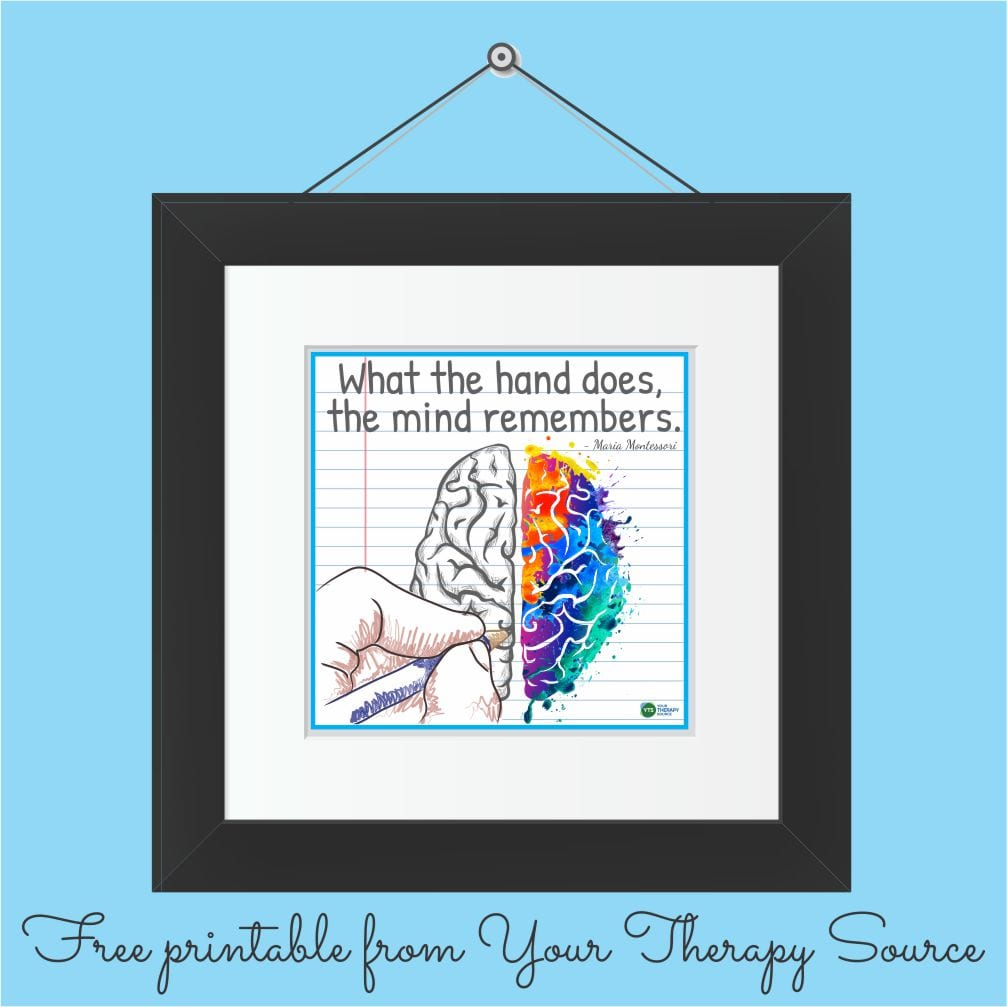
\includegraphics[width=5cm]{P2023.AIBCCSS.ExtendedMindDistributedCognitionSystemicThinking/what-the-hand-does-the-mind-remembers.jpg}
 
 \end{center}

\begin{center}
\tiny
Reference: Robert MacDougall, ``The Significance of the Human Hand in the Evolution of Mind,'' The American Journal of Psychology, 16(2):232 -- 242, Apr., 1905\\Picture taken from \url{https://www.yourtherapysource.com/blog1/2019/02/07/3-evidence-based-benefits-of-writing-by-hand/}.
\end{center}
\end{frame}


\begin{frame}
{\centerline{Extended Mind (1/2)}}

\begin{itemize}
    \item Let us consider a simple problem: we are given shapes and we have to see if they fit holes:
\end{itemize} 

\begin{center}
 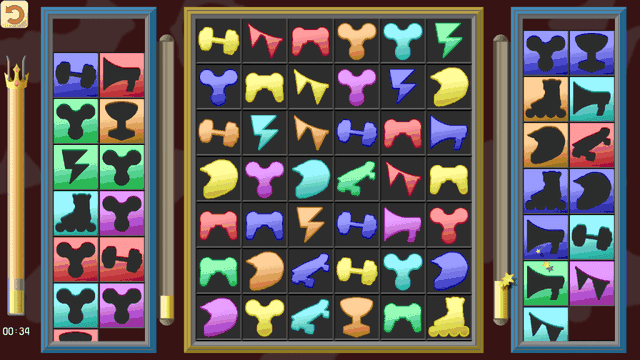
\includegraphics[width=8cm]{P2023.AIBCCSS.ExtendedMindDistributedCognitionSystemicThinking/campaignlevel-3-f53c.png}
 
 \end{center}

\begin{center}
    \tiny{Source of the content: Andy Clark and David Chalmers, ``The extended mind,'' Analysis 58 (1): 7--19 , 1998 \\Picture taken from \url{https://gurugamer.com/mobile-games/shapes-and-holes-a-new-mobile-puzzler-where-you-fit-things-into-other-things-1214}.}
\end{center}
\end{frame}


\begin{frame}
{\centerline{Extended Mind (2/2)}}
\begin{itemize}
    \item Let us consider three cases:
    \begin{itemize}
        \item this is a computer game (as in the picture) and the person has to rotate the pieces by mind and determines the fitting;
        \item this is a paper game and the person has pieces that s/he rotates manually to determine the fit;
        \item let us assume that the person has an implanted device, say, special smart glasses, that perform the rotation and then s/he just does the fitting
    \end{itemize}
    \item What is the level of cognition present in these cases?
        \begin{itemize}
   		 \item Clark and Chalmers claim that it is the same.
        \end{itemize}
    \item Therefore, what is the boundary of our mind?
\end{itemize} 
\begin{center}
    \tiny{Source of the content: Andy Clark and David Chalmers, ``The extended mind,'' Analysis 58 (1): 7--19 , 1998}
\end{center}

\end{frame}

\begin{frame}
{\centerline{Tools and Mind}}
\begin{itemize}
    \item There are many tools even before computer that helped our cognitive tasks
    \begin{itemize}
        \item abacus
        \item paper and pen
        \item sliding rule
        \item $\ldots{}$
            \end{itemize}
    \item Once we start using it, they become intrinsic part of our reasoning and computational process
    \item Think at how we do computations in column
           \begin{itemize}
        		\item papers and pen are essential components of our reasoning process
		\item even when we do the computation in our mind we often simulate the presence of paper and pen
	   \end{itemize} 
    \item Once more, \textcolor{orange}{\bf what are the boundaries of our mind}?
\end{itemize} 

\begin{center}
    \tiny{Source of the content: Andy Clark and David Chalmers, ``The extended mind,'' Analysis 58 (1): 7--19 , 1998}
\end{center}

\end{frame}

\begin{frame}
{\centerline{Impact}}
\begin{itemize}
    \item We care about this for at least three reasons:
    \begin{itemize}
        \item we understand that the request of tools may be not a caprice of a spoiled kid but an actual desire to organize the (extended) mind in the most effective way
        \item when developing tools we need to think at how such tools can most effectively ``extend'' the mind of the users, and not simply being tools
        \item when creating a (development) environment for us and for our people we must determine the best configuration
    \end{itemize}
    \item Once more, \textcolor{orange}{\bf what are the boundaries of our mind}?
\end{itemize} 

\begin{center}
    \tiny{Source of the content: Andy Clark and David Chalmers, ``The extended mind,'' Analysis 58 (1): 7--19 , 1998}
\end{center}

\end{frame}

\begin{frame}
{\centerline{Active Externalism}}
\begin{itemize}
    \item The claim of Clark and Chalmers is that the tool and the person couple together forming a unique mix
    \item The external tools are not just instruments for actions that are determined in an hypothesized internal mind
    \item Rather, they are a key active external component of our mind, hence we talk of:
    \begin{itemize}
    \item \textcolor{red}{Active Externalism}
\end{itemize} 
     \item Think at exoskeleton, for instance 
\end{itemize} 

\begin{center}
    \tiny{Source of the content: Andy Clark and David Chalmers, ``The extended mind,'' Analysis 58 (1): 7--19 , 1998}
\end{center}

\end{frame}

\begin{frame}
{\centerline{Example: Exoskeleton}}

\begin{itemize}
    \item A Hybrid Assistive Limb:
\end{itemize} 

\begin{center}
 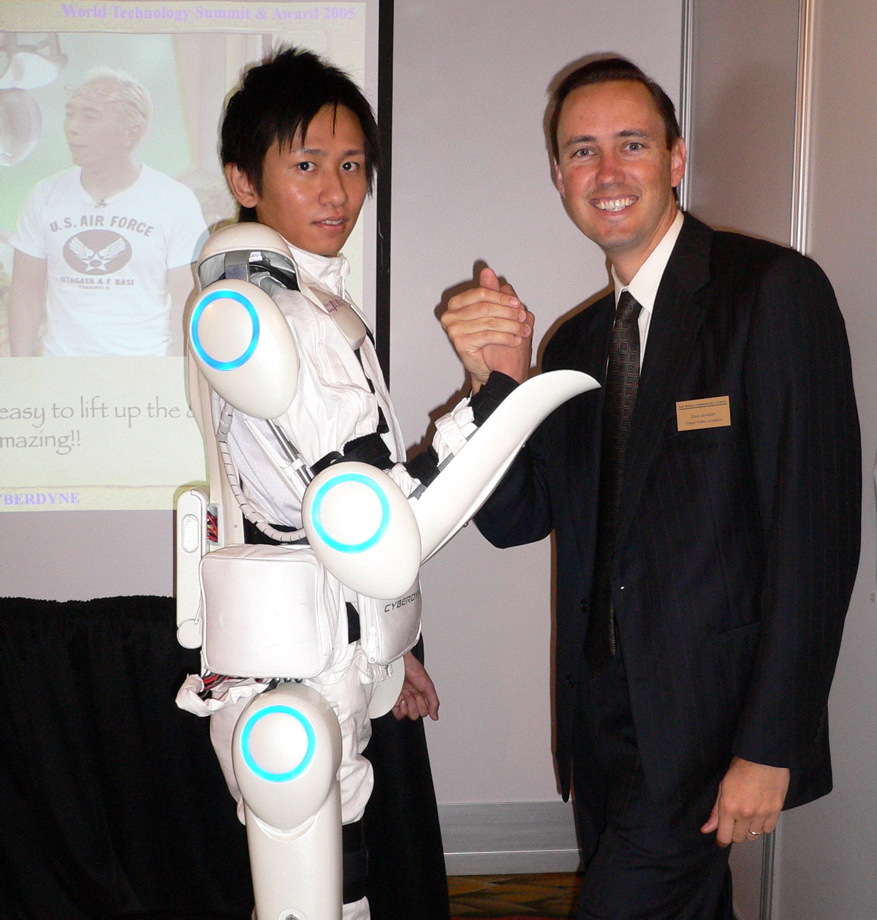
\includegraphics[width=4cm]{P2023.AIBCCSS.ExtendedMindDistributedCognitionSystemicThinking/Hybrid_Assistive_Limb.jpg}
 
 \end{center}
 
 \begin{itemize}
 \item ``The external features here are just as causally relevant as typical internal features of the brain'' Clark and Chalmers.
 \end{itemize}
 
\begin{center}
    \tiny{Picture taken from \url{https://en.wikipedia.org/wiki/Powered_exoskeleton}. Statement from Andy Clark and David Chalmers, ``The extended mind,'' Analysis 58 (1): 7--19 , 1998.}
\end{center}
\end{frame}

\begin{frame}
{\centerline{Beliefs}}
\begin{itemize}
    \item The mind is also the center of our beliefs
    \item Typically we think at beliefs as something completely internal to our mind
    \item Is it really so?
     \item Or think at how many interaction with an environment of tools and devices we would need to think if we would assume that:
         \begin{itemize}
    \item processes are only inside the body and 
    \item everything is is something that is manipulated and ``used''
\end{itemize} 
\end{itemize} 

\begin{center}
    \tiny{Source of the content: Andy Clark and David Chalmers, ``The extended mind,'' Analysis 58 (1): 7--19 , 1998}
\end{center}

\end{frame}

\begin{frame}
{\centerline{Cognition and consciousness}}
\begin{itemize}
    \item Cognition is not consciousness
    \item Remember of the emotional long term memory or even at the procedural long term memory
    \item And think at all the work, for instance of therapists of moving feelings at the consciousness level 
    \item Discussing consciousness is beyond the purpose of this course
\end{itemize} 

\begin{center}
 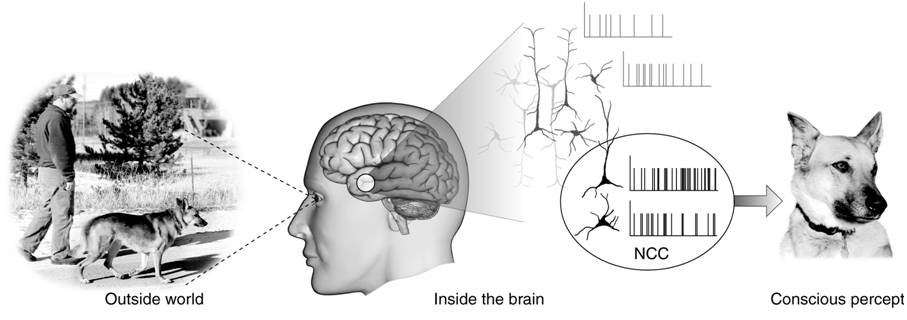
\includegraphics[width=10cm]{P2023.AIBCCSS.ExtendedMindDistributedCognitionSystemicThinking/Neural_Correlates_Of_Consciousness.jpg}
 
 \end{center}

\begin{center}
 \tiny{Picture taken from \url{https://en.wikipedia.org/wiki/Consciousness} where it is credited to Christof Koch (\url{https://en.wikipedia.org/wiki/Christof_Koch}).}
 \end{center}

\end{frame}

\begin{frame}
{\centerline{Location of our beliefs (1/3)}}
\begin{itemize}
    \item Let us consider these two cases (from the reference):
    \begin{itemize}
    \item Inga wants to go to the MoMA and remembers that it is on 11 West 53 Street, Manhattan, and she goes there
        \begin{itemize}
    \item She had a (previous) belief  \textcolor{red}{in her \textbf{mind}} about the location and she uses it to direct her actions
    \end{itemize} 
    \item Otto suffers from Alzheimer diseases, so he forgets what he learns and to overcome this he takes with him a tablet where marks down information
    \item Also Otto wants to go to the MoMA, he looks it up in the tablet, finds that it is on 11 West 53 Street, Manhattan, and goes there
            \begin{itemize}
    \item He had a (previous) belief  about the location \textcolor{cyan}{in his the \textbf{tablet}} and he uses it to direct her actions
    \end{itemize} 
    \item What is the difference?
\end{itemize} 
\end{itemize} 

\begin{center}
    \tiny{Source of the content: Andy Clark and David Chalmers, ``The extended mind,'' Analysis 58 (1): 7--19 , 1998}
\end{center}

\end{frame}

\begin{frame}
{\centerline{Location of our beliefs (2/3)}}
\begin{itemize}
    \item We could explain the reasoning process of Otto in terms of external tools, but it would be quite convoluted
    \item For Otto the tablet plays the same role as the \textcolor{red}{\it mind} for Inga
    \item For beliefs what matter is not where they are located but the role that they play
    \item After all, in what the beliefs of Otto and of Inga differ?
  \begin{itemize}
    \item  Their only difference is in the physical location
\end{itemize} 
\item There could be additional counterclaims of the differences on beliefs:
\item \textcolor{orange}{The tablet of Otto could not be always with him for instance when he takes a shower}
  \begin{itemize}
    \item \textcolor{blue}{Inga beliefs could also be our her if she is drunk or excited}
\end{itemize} 
\end{itemize} 

\begin{center}
    \tiny{Source of the content: Andy Clark and David Chalmers, ``The extended mind,'' Analysis 58 (1): 7--19 , 1998}
\end{center}

\end{frame}

\begin{frame}
{\centerline{Location of our beliefs (3/3)}}
\begin{itemize}
\item  \textcolor{orange}{Otto could be slower in gathering the information}
  \begin{itemize}
    \item \textcolor{blue}{What if Inga had a memory disorder that requires her a slow process to recall her beliefs?}
\end{itemize} 
\item  \textcolor{orange}{The process of Otto requires perception while the one of Inga only introspection}
  \begin{itemize}
    \item \textcolor{blue}{Are we sure that when we look up information on a table we are really exercising perception? If we consider the tablet as part of the mind, the process is still introspective}
\end{itemize} 
\item There are no strong arguments against considering also the one of Otto as a belief, and thus that his minds extends to the tablet
\end{itemize} 

\begin{center}
    \tiny{Source of the content: Andy Clark and David Chalmers, ``The extended mind,'' Analysis 58 (1): 7--19 , 1998}
\end{center}

\end{frame}

\begin{frame}
{\centerline{Additional speculation on Otto}}
\begin{itemize}
\item The tablet is an integral part of the life of Otto
\item Otto can access directly and without any problem the information there
\item Otto accepts as true the information stored in the notebook automatically
\item Otto has once validated such information, and since then such information is valid
\begin{itemize}
\item \textcolor{orange}{What if someone leaks inside the table and put there wrong information?}
\item \textcolor{blue}{Well, if someone by some subliminal manipulation forces in the mind some wrong information?}
\end{itemize} 
\end{itemize} 


\begin{center}
    \tiny{Source of the content, also copied verbatim: Andy Clark and David Chalmers, ``The extended mind,'' Analysis 58 (1): 7--19 , 1998}
\end{center}

\end{frame}

\begin{frame}
{\centerline{Can we extend this concept beyond?}}
\begin{itemize}
\item What about groups of people, where the knowledge is distributed?
\item The key point is how much our belief is:
\begin{itemize}
\item trust
\item reliance
\item availability 
\end{itemize} 
\item indeed, the language pays a major role, but ...
\end{itemize} 

\begin{center}
    \tiny{Source of the content, also copied verbatim: Andy Clark and David Chalmers, ``The extended mind,'' Analysis 58 (1): 7--19 , 1998}
\end{center}

\end{frame}


\begin{frame}
{\centerline{Communication means (1/3)}}

\begin{itemize}
\item Empirical studies with 38 IT professionals
\item Analysis of the communication patterns
\end{itemize} 

\begin{center}
\textbf{When the communication is considered positive}
\end{center}

\begin{center}
\begin{tabular}{|c|c|c|c|}
\toprule
\textbf{What is being used} & \textbf{by me} & \textbf{by others} & \textbf{by any}\\
\midrule Vocalics & 16\% & 16\% & 26\% \\
\midrule Kinesics & 21\% & 8\% & 24\% \\
\midrule Chronemics & 3\% & 5\% & 5\%\\
\midrule Proxemics & 0\% & 3\% & 3\%\\
\midrule Oculesics &  0\% & 0\% & 0\%\\
\midrule Synchrony & 3\% & 0\% & 3\%\\
\bottomrule
\end{tabular}
\end{center}

\begin{center}
    \tiny{Source: Paolo Ciancarini, Mirko Farina, Sergey Masyagin, Giancarlo Succi, Sofiia Yermolaieva, and Nadezhda Zagvozkina. ``Non verbal communication in software engineering - an empirical study.'' IEEE Access, 9:71942–71953, 2021}
\end{center}

\end{frame}


\begin{frame}
{\centerline{Communication means (2/3)}}

\begin{center}
\textbf{When the communication is considered negative}
\end{center}

\begin{center}
\centering
\begin{tabular}{|c|c|c|c|}
\midrule
{\textbf{What is being used}} & {\textbf{by me}} & \textbf{by others} & \textbf{by any}\\
\midrule
{Vocalics} & 5\% & 8\% & 11\% \\
\midrule
{Kinesics} & 11\% & 5\% & 11\% \\
\midrule
{Chronemics} & 8\% & 8\% & 16\%\\
\midrule
{Proxemics} & 0\% & 3\% & 3\%\\
\midrule
{Oculesics} &  0\% & 3\% & 3\%\\
\midrule
 {Synchrony} & 5\% & 0\% & 5\%\\
\midrule
\end{tabular}
\end{center}

\begin{center}
    \tiny{Source: Paolo Ciancarini, Mirko Farina, Sergey Masyagin, Giancarlo Succi, Sofiia Yermolaieva, and Nadezhda Zagvozkina. ``Non verbal communication in software engineering - an empirical study.'' IEEE Access, 9:71942–71953, 2021}
\end{center}

\end{frame}


\begin{frame}
{\centerline{Communication means (3/3)}}

\begin{itemize}
\item When the communication is positive:
\begin{itemize}
\item There is a larger incidence of vocalics and kinetics
\item When the communication is negative people think that time is wasted 
\end{itemize}
\item Chronemics play a major role in meetings:
\begin{itemize}
\item When the communication is negative they are remarkably noted 
\item When the communication is positive people feel them implicitly (coded in comments)
\end{itemize}

\end{itemize}

\begin{center}
    \tiny{Source: Paolo Ciancarini, Mirko Farina, Sergey Masyagin, Giancarlo Succi, Sofiia Yermolaieva, and Nadezhda Zagvozkina. ``Non verbal communication in software engineering - an empirical study.'' IEEE Access, 9:71942–71953, 2021}
\end{center}

\end{frame}

\begin{frame}
{\centerline{Systemic Thinking (1/2)}}

\begin{itemize}
\item Systemic thinking is an interdisciplinary field of research that 
\begin{itemize}
\item attempts to comprehend complex human (and non-human) structures
\item by explaining their mutual interconnections from a holistic standpoint
\end{itemize}
\item It is an approach applied in many disciplines, including sociology, psychology, management, etc
\item An idea inspired somehow by many Eastern philosophies
\item There are elements also in Pythagorean theories, then going to Plato, Avicenna (Ibn Sina), $\ldots{}$
\end{itemize}

\begin{center}
    \tiny{Source: Mirco Farina, Giancarlo Succi, Ananga Thapaliya. ``A Systemic Perspective on Software Engineering.'' Under review}
\end{center}

\end{frame}

\begin{frame}
{\centerline{Systemic Thinking (2/2)}}

\begin{itemize}
\item Systemic thinking draws from different disciplines  (engineering, computer science,  cognitive science,  management, philosophy, psychology, biology, ...)
\begin{itemize}
\item  it attempts to provide a discipline-agnostic approach for dealing with complex  problems
\item  to understand the structure and properties of a given system in terms of the relationships among its components
\end{itemize}
\item It was introduced in software engineering in 1971 by Weinberg (``The psychology of computer programming'') and then forgotten or declassed under the term \textit{peopleware}
\item The agile proponents of the division between tame and wicked problems were apparently unaware of systemic thinking.
\end{itemize}

\begin{center}
    \tiny{Source: Mirco Farina, Giancarlo Succi, Ananga Thapaliya. ``A Systemic Perspective on Software Engineering.'' Under review}
\end{center}

\end{frame}

\begin{frame}
{\centerline{Systemic Thinking and Software Engineering}}
\begin{itemize}
    \item Systemic thinking in software engineering views the software development process as a complex and dynamic system composed of multiple interconnected parts.
    \begin{itemize}
    \item it emphasizes the interdependences of individuals, teams, and organizations, and 
    \item how each interdepencency influences and are influenced by one another 
    \item also identifying coherences and incoherences in representations and
    \item (self-)contradicting thought
    \item schismogenesis
\end{itemize} 
    \item Can be divided into psychological and sociological systemic thinking
\end{itemize} 

\begin{center}
    \tiny{Source: Mirco Farina, Giancarlo Succi, Ananga Thapaliya. ``A Systemic Perspective on Software Engineering.'' Under review}
\end{center}

\end{frame}

\begin{frame}
{\centerline{Sociological and Psychological Views}}

\begin{center}
 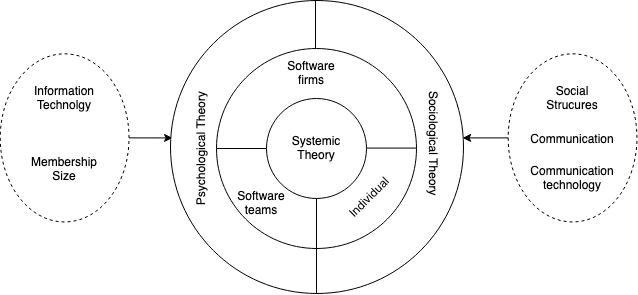
\includegraphics[width=12cm]{P2023.AIBCCSS.ExtendedMindDistributedCognitionSystemicThinking/SociologicalPsychologicalST.png}
 
 \end{center}

\begin{center}
    \tiny{Picture from an earlier version of the paper: Mirco Farina, Giancarlo Succi, Ananga Thapaliya. ``A Systemic Perspective on Software Engineering.'' Under review}
 \end{center}

\end{frame}

\begin{frame}
{\centerline{Example of Systemic Analysis (1/2)}}

\begin{center}
 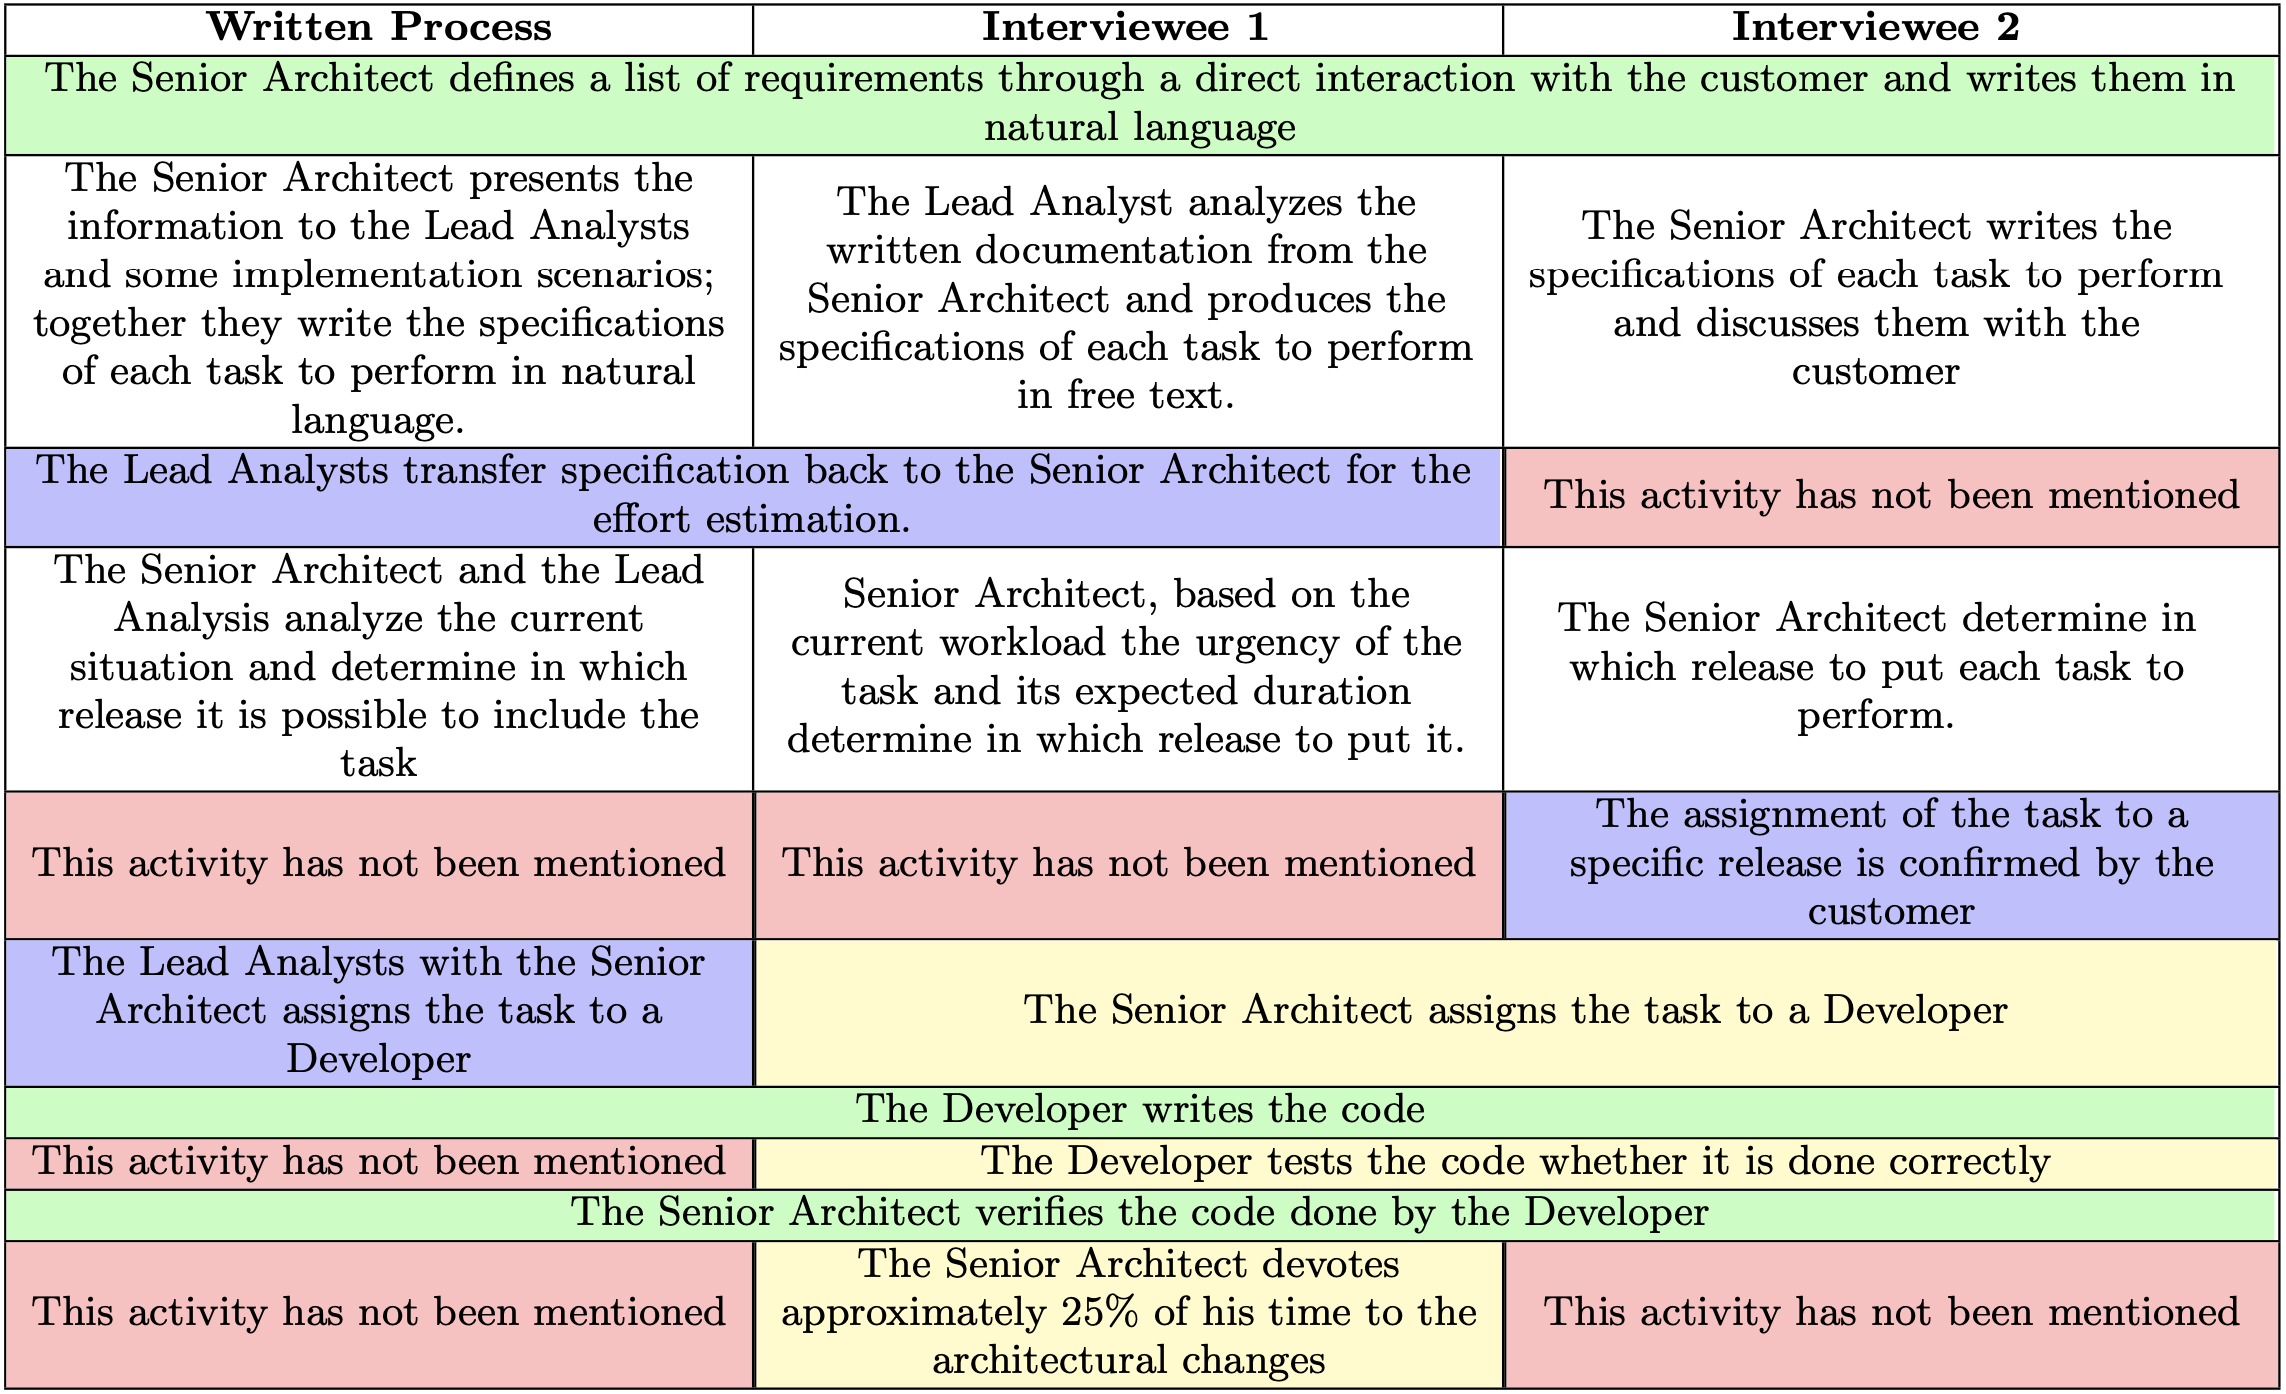
\includegraphics[width=10cm]{P2023.AIBCCSS.ExtendedMindDistributedCognitionSystemicThinking/ExampleSystemicAnalysis.jpg}
 
 \end{center}

\begin{center}
    \tiny{Picture from: Vladimir Ivanov, Manuel Mazzara, Witold Pedrycz, Alberto Sillitti, and Giancarlo Succi. ``Assessing the Process of an Eastern European Software SME Using Systemic Analysis, GQM, and Reliability Growth Models: A Case Study.'' In Proceedings of the 38th International Conference on Software Engineering Companion (ICSE 2016), pages 251–259, Austin, Texas, May 2016. ACM}
 \end{center}

\end{frame}

\begin{frame}
{\centerline{Example of Systemic Analysis (2/2)}}

\begin{center}
 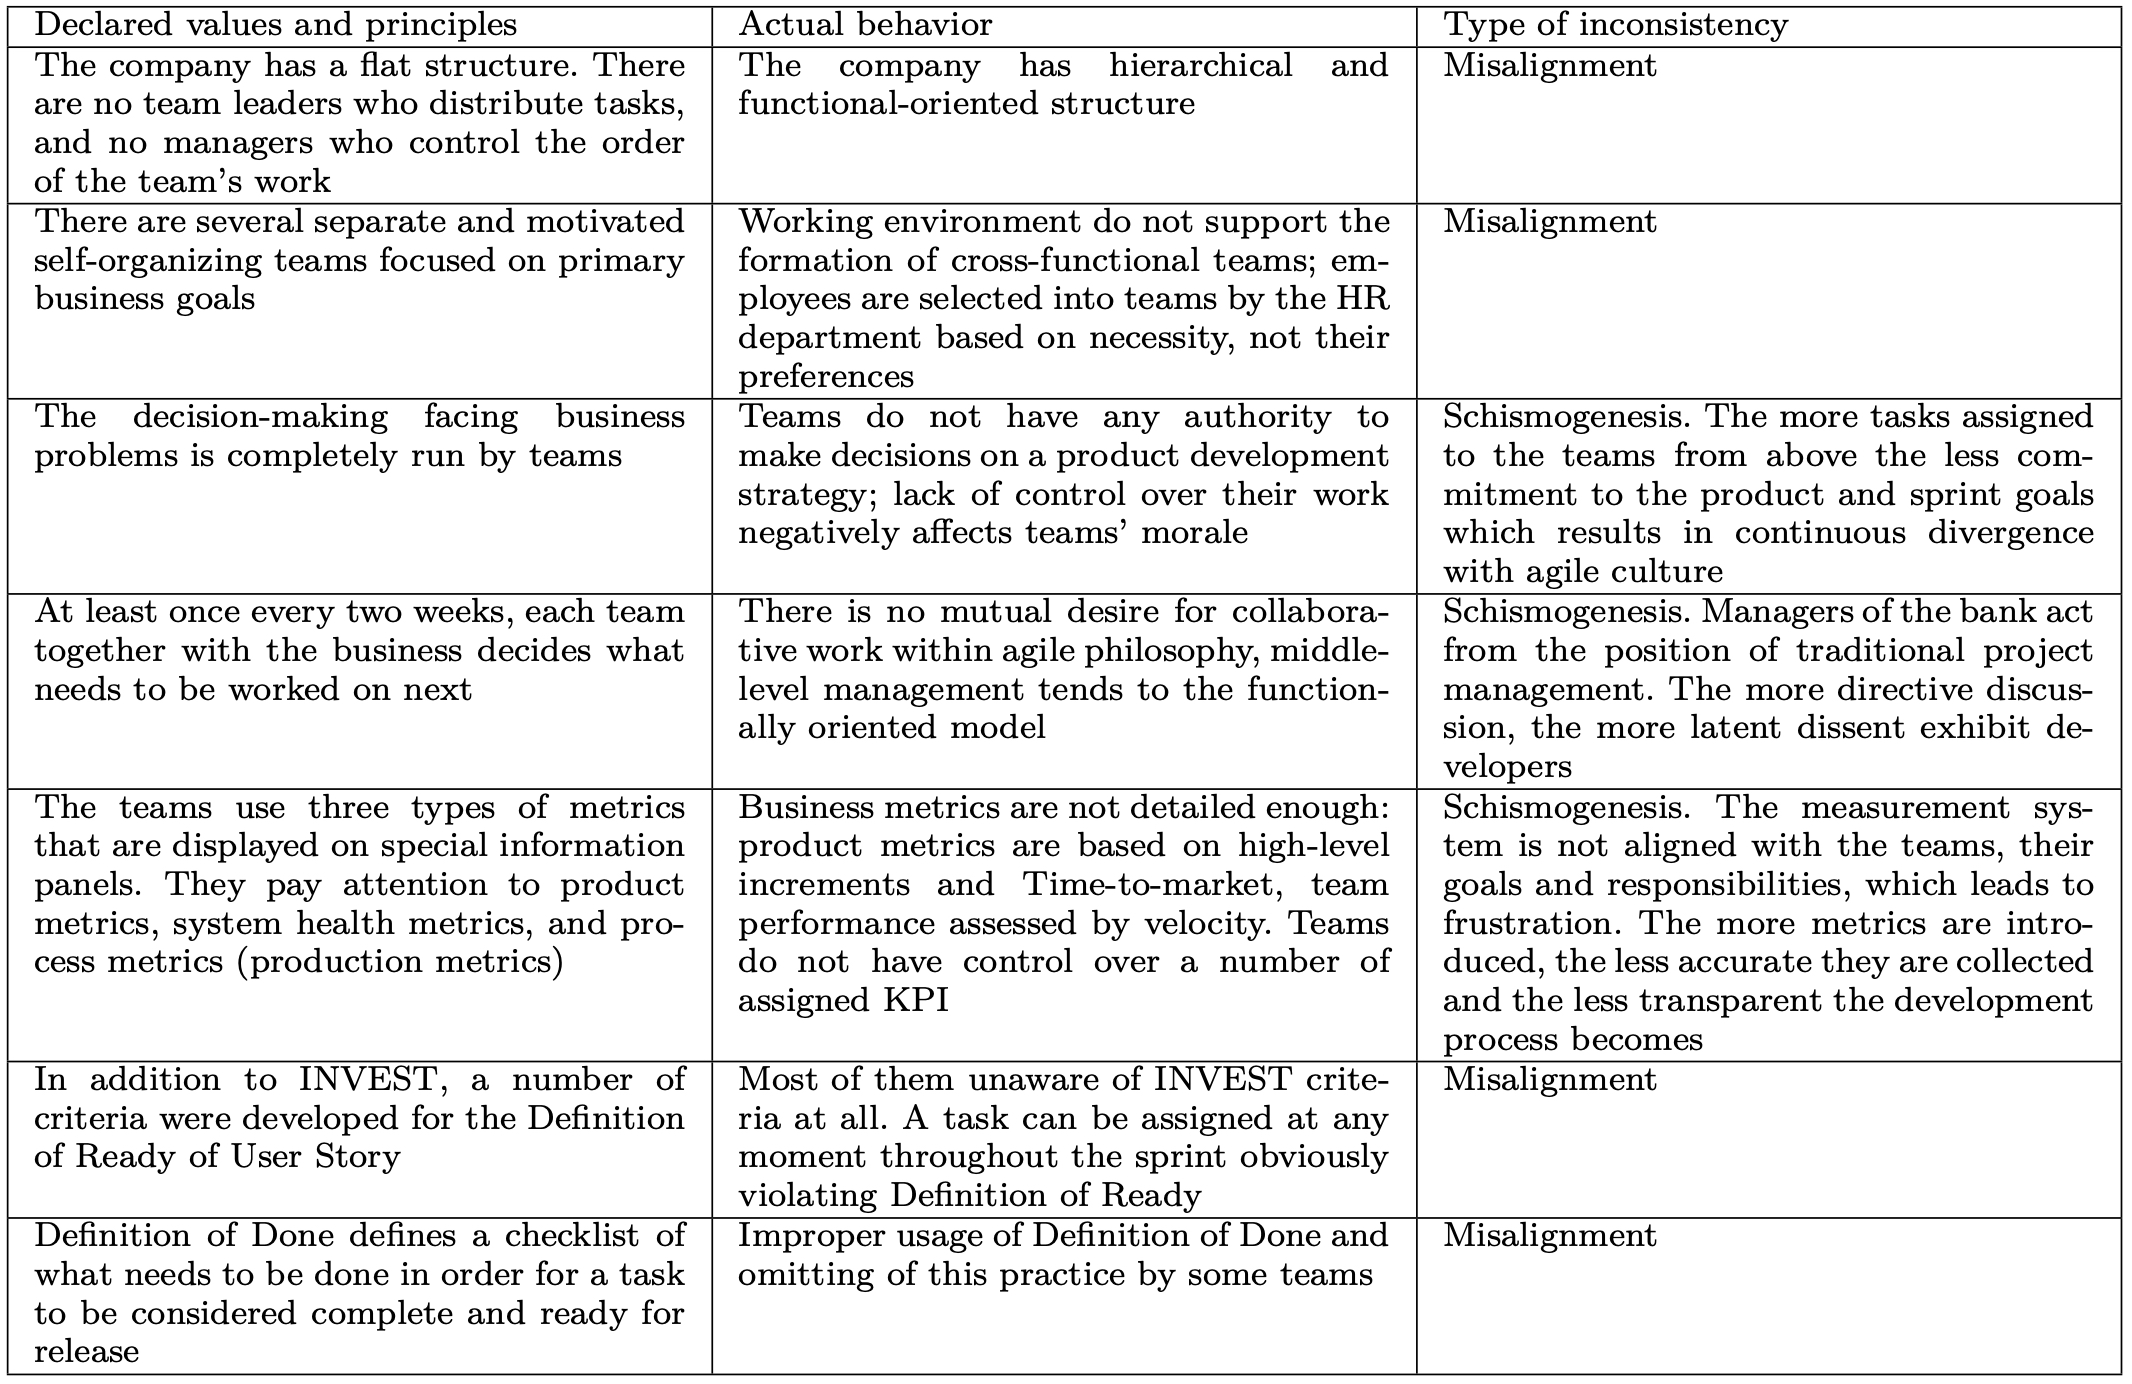
\includegraphics[width=10cm]{P2023.AIBCCSS.ExtendedMindDistributedCognitionSystemicThinking/AkBars-Systemic.jpg}
 
 \end{center}

\begin{center}
    \tiny{Picture from: Merab Gogichaty, Vladimir Ivanov, Artem Kruglov, Witold Pedrycz, Aliya Samatova, Giancarlo Succi, Raphael Valeev, ``A Systemic Approach to Evaluating the Organizational Agility in Large-Scale Companies,'' in IEEE Access, vol. 11, pp. 3307-3323, 2023}
 \end{center}

\end{frame}


\begin{frame}
{\centerline{Empirical Study (1/2)}}

\begin{itemize}
 \item Core question: How can the application of systemic thinking help us understand how software teams work and operate in their daily practice?
\item Phase 1: Online questionnaire on to 50 software developers working in Russia, Nepal, and Luxembourg based on closed questions
    \begin{itemize}
    \item Overall result: \textcolor{red}{systemic thinking is deeply ingrained in the daily activities of software engineers}
    \end{itemize}
\end{itemize}


\begin{center}
    \tiny{Source: Mirco Farina, Giancarlo Succi, Ananga Thapaliya. ``A Systemic Perspective on Software Engineering.'' Under review}
\end{center}

\end{frame}

\begin{frame}
{\centerline{Empirical Study (2/2)}}

\begin{itemize}
\item Phase 2: Refinement of Phase 1 with physical interviews with 11 expert Russian programmers and managers based on open questions
\begin{itemize}
    \item Overall result: \textcolor{red}{psychological and sociological systemic approaches should be considered in all software engineering practices} and 
    \item  \textcolor{red}{an improved understanding of these systemic approaches would benefit all the roles in any team}
    \end{itemize}
\item overall, the most commonly stated terms have to do with communication, teamwork, and social leadership. 
\begin{itemize}
\item i.e, software engineering is a social phenomenon that is heavily impacted by group dynamics and individual personalities --- more on distributed cognition
\end{itemize}
\end{itemize}


\begin{center}
    \tiny{Source: Mirco Farina, Giancarlo Succi, Ananga Thapaliya. ``A Systemic Perspective on Software Engineering.'' Under review}
\end{center}

\end{frame}

\begin{frame}
{\centerline{Systemic Thinking and Agility (1/2)}}

\begin{itemize}
\item Another empirical study
\item Questions: 
\begin{itemize} 
\item Do software engineers have a high level
of systemic thinking in general?
\item What is the level of systemic thinking in the different processes (traditional, agile, mix agile-traditional, ad-hoc)?
\end{itemize}
\item Online questionnaire with 101 respondents worldwide 
\item Using the Systemic Thinking Scale to measure the level of systemic thinking (from 0 to 80)
\end{itemize}

\begin{center}
    \tiny{Source: Paolo Ciancarini, Mirco Farina, Giancarlo Succi, Ananga Thapaliya. ``Systemic thinking and software development processes.'' Under review}
\end{center}

\end{frame}

\begin{frame}
{\centerline{Systemic Thinking and Agility (2/2)}}

\begin{center}
\begin{tabular}{|l|l|l|l|}
\midrule
\textbf{Process}             & \textbf{Average} &  \textbf{Stdev} &  \textbf{Score} \\ \midrule
Agile       & 2.78 & 0.17    & 55.66 \\ \midrule
Mixed  & 2.75 & 0.29    & 54.95 \\ \midrule
Traditional   & 2.74  & 0.32   & 54.75 \\ \midrule
Ad hoc            & 2.49 & 0.29    & 49.89 \\ \midrule
\end{tabular}

\end{center}
\begin{itemize}
\item In terms of significance:
\begin{itemize}
    \item agile and mixed have a probability of mean STS not different from ad-hoc of 1.1\%,
    \item traditional not different from ad-hoc of 7.1\%
    \item traditional and mixed are almost indistinguishable one another in terms of STS
\end{itemize}
\end{itemize}

\begin{center}
    \tiny{Source: Paolo Ciancarini, Mirco Farina, Giancarlo Succi, Ananga Thapaliya. ``Systemic thinking and software development processes.'' Under review}
\end{center}

\end{frame}


 
\begin{frame}
{\centerline{Toward Distributed Cognition}}

\begin{itemize}
\item We have seen that:
\begin{itemize}
    \item cognitive processes may extend to tools we are interacting with
\end{itemize}
\item However
\begin{itemize}
    \item cognitive processes may also \textcolor{red}{span through multiple individuals}
    \item cognitive processes may also \textcolor{cyan}{cross time boundaries}
\end{itemize}
\end{itemize}

\begin{center}
    \tiny{Source: James Hollan, Edwin Hutchins, and David Kirsh. 2000. ``Distributed cognition: toward a new foundation for human-computer interaction research.'' ACM Trans. Comput.-Hum. Interact. 7, 2 (June 2000), 174–196}
\end{center}

\end{frame}

\begin{frame}
{\centerline{Cognitive Architectures}}

\begin{itemize}
\item We have seen that:
\begin{itemize}
    \item cognitive processes define paths for the information to flow
    \item during these path the information is transmitted and/or transformed
    \item this network defines the \textcolor{red}{cognitive architecture}  
\end{itemize}
\item Now:
\begin{itemize}
    \item social organizations structure how the information flow in a group of people and devices 
    \item therefore \textcolor{cyan}{\bf social organizations can be considered cognitive architectures themselves}
\end{itemize}
\end{itemize}

\begin{center}
    \tiny{Source: James Hollan, Edwin Hutchins, and David Kirsh. 2000. ``Distributed cognition: toward a new foundation for human-computer interaction research.'' ACM Trans. Comput.-Hum. Interact. 7, 2 (June 2000), 174–196}
\end{center}

\end{frame}

\begin{frame}
{\centerline{Distributed Cognition}}

\begin{itemize}
\item Given that social organizations can be considered cognitive architectures
\begin{itemize}
    \item we can use the dynamics of social groups to explain what passes to the minds \textcolor{red}{(of people?)} 
    \item and here we are understanding what phenomenologically we appreciated with systemic analysis
 \end{itemize}
    \item we can conclude that also \textcolor{cyan}{the cognitive process of an individual is distributed}  
\end{itemize}

\begin{center}
    \tiny{Source: James Hollan, Edwin Hutchins, and David Kirsh. 2000. ``Distributed cognition: toward a new foundation for human-computer interaction research.'' ACM Trans. Comput.-Hum. Interact. 7, 2 (June 2000), 174–196}
\end{center}

\end{frame}

\begin{frame}
{\centerline{Three fundamental questions}}

\begin{enumerate}
\item How groups of people implement cognitive processes that we usually consider belonging to an individual mind?\newline
    \item What are the differences of the cognitive process of a group as a whole from the cognitive process of the people in the group?\newline
    \item How is an individual cognitive processed affected by participating in a group cognitive process?\newline
\end{enumerate}

\begin{center}
    \tiny{Source: James Hollan, Edwin Hutchins, and David Kirsh. 2000. ``Distributed cognition: toward a new foundation for human-computer interaction research.'' ACM Trans. Comput.-Hum. Interact. 7, 2 (June 2000), 174–196}
\end{center}

\end{frame}

\begin{frame}
{\centerline{The role of culture}}

\begin{enumerate}
\item How groups of people implement cognitive processes that we usually consider belonging to an individual mind?\newline
    \item What are the differences of the cognitive process of a group as a whole from the cognitive process of the people in the group?\newline
    \item How is an individual cognitive processed affected by participating in a group cognitive process?\newline
\end{enumerate}

\begin{center}
    \tiny{Source: James Hollan, Edwin Hutchins, and David Kirsh. 2000. ``Distributed cognition: toward a new foundation for human-computer interaction research.'' ACM Trans. Comput.-Hum. Interact. 7, 2 (June 2000), 174–196}
\end{center}

\end{frame}

\begin{frame}
{\centerline{Cognitive Ethnography}}

\begin{itemize}
\item If the structure of the society defines the cognitive architecture
\begin{itemize}
\item then \textcolor{red}{understanding the underlying culture has a pivotal role in determining the cognitive process}
\end{itemize}
\item the culture defines the cognitive process of the societies and the people living in it
\item and inside the culture there are the specific environments with typical learning processes, problem solving approaches, reasoning mechanisms
\item Therefore cognition crosses the boundaries of time
\begin{itemize}
\item to understand cognition we need \textcolor{cyan}{\textbf{cognitive ethnography}}
\end{itemize}
\end{itemize}


\begin{center}
    \tiny{Source: James Hollan, Edwin Hutchins, and David Kirsh. 2000. ``Distributed cognition: toward a new foundation for human-computer interaction research.'' ACM Trans. Comput.-Hum. Interact. 7, 2 (June 2000), 174–196}
\end{center}

\end{frame}

\begin{frame}
{\centerline{The role of the cognitive architecture}}

\begin{itemize}
\item The cognitive architecture is the root of the mind of the organization:
\begin{itemize}
\item it is composed by people and tools
\item it is what differentiate different development processes
\end{itemize}
\item failing to implement a development process often means failing to shape the cognitive architecture in the desired way and, consequently
\begin{itemize}
\item \textcolor{cyan}{understanding the cognitive architecture is the most effective way to enact effective development processes}
\end{itemize}
\item when agile methods refer to \textcolor{red}{emerging structure} of an organization the refer (often unknowingly) to making evident underlying cognitive architecture
\end{itemize}

\end{frame}

\begin{frame}
{\centerline{Ethnography means $\ldots{}$}}

\begin{itemize}
\item Experimentation is not just formal experiments
\item Ethnography: understanding \textcolor{red}{being inside}; it depends on
\begin{itemize}
\item the ability of the scientist to \textcolor{cyan}{immerge into the reality} and \textcolor{orange}{feel the experience} but still provide a
\item  \textcolor{blue}{reliable account} of it understanding the own subjectivity
\end{itemize}
\end{itemize}


\begin{center}
 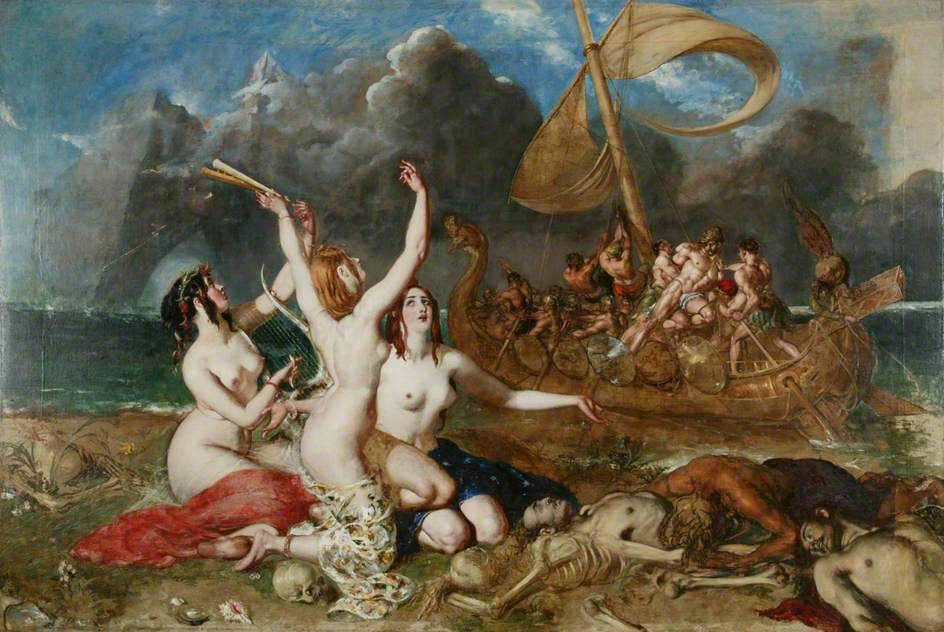
\includegraphics[width=6cm]{P2023.AIBCCSS.ExtendedMindDistributedCognitionSystemicThinking/The_Sirens_and_Ulysses_by_William_Etty.jpg}
 
 \end{center}

\begin{center}
    \tiny{The drawing is ``The Sirens and Ulysses'' by William Etty (1837) taken from \url{https://en.wikipedia.org/wiki/File:The_Sirens_and_Ulysses_by_William_Etty,_1837.jpg}}
 \end{center}

\end{frame}


\begin{frame}
{\centerline{Understanding the cognitive architecture}}

\begin{center}
 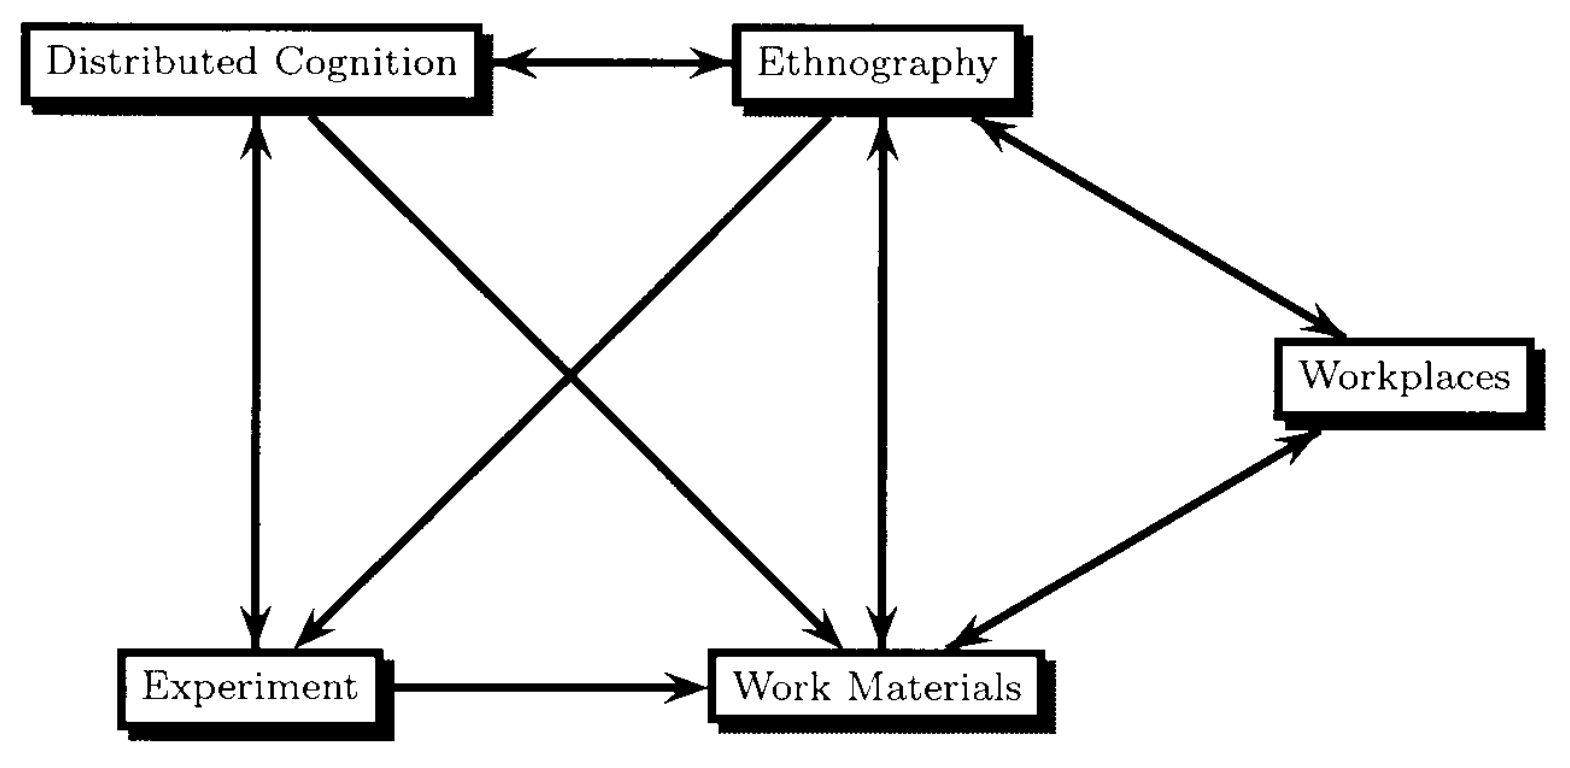
\includegraphics[width=10cm]{P2023.AIBCCSS.ExtendedMindDistributedCognitionSystemicThinking/networkDistributedCognition.jpg}
 
 \end{center}

\begin{center}
 \tiny{Picture taken from James Hollan, Edwin Hutchins, and David Kirsh. 2000. ``Distributed cognition: toward a new foundation for human-computer interaction research.'' ACM Trans. Comput.-Hum. Interact. 7, 2 (June 2000), pag. 181}
 \end{center}

\end{frame}


\begin{frame}
{\centerline{Evidences of Distributed Cognition}}

\begin{itemize}
\item And of cognitive architectures:
\begin{itemize}
\item The crew in a ship creating together a unique ``computational'' entity
\item The pilots in a plane working together and with tools
\item A group of fishermen also on different ships
\end{itemize}
\item There are also multiple communication mechanisms
\item This has also a strong impact on how to design HCI in computers
\end{itemize}
\begin{center}
    \tiny{Source: James Hollan, Edwin Hutchins, and David Kirsh. 2000. ``Distributed cognition: toward a new foundation for human-computer interaction research.'' ACM Trans. Comput.-Hum. Interact. 7, 2 (June 2000), 174–196}
\end{center}

\end{frame}



\begin{frame}
{\centerline{Questions?}}
\vspace{1cm}
\begin{center}
    \LARGE{Thank you for your time.}
\end{center}

\end{frame}


\end{document}
